\documentclass[paper=a4 wide, fontsize=12pt]{scrartcl} 

\usepackage[T1]{fontenc} % Use 8-bit encoding that has 256 glyphs
\usepackage{fourier} % Use the Adobe Utopia font for the document - comment this line to return to the LaTeX default
\usepackage[english]{babel} % English language/hyphenation
\usepackage{amsmath,amsfonts,amsthm} % Math packages

\usepackage{lipsum} % Used for inserting dummy 'Lorem ipsum' text into the template

\usepackage{sectsty} % Allows customizing section commands
\allsectionsfont{\centering \normalfont\scshape} % Make all sections centered, the default font and small caps

\usepackage{fancyhdr} % Custom headers and footers
\pagestyle{fancyplain} % Makes all pages in the document conform to the custom headers and footers
\fancyhead{} % No page header - if you want one, create it in the same way as the footers below
\fancyfoot[L]{} % Empty left footer
\fancyfoot[C]{} % Empty center footer
\fancyfoot[R]{\thepage} % Page numbering for right footer
\renewcommand{\headrulewidth}{0pt} % Remove header underlines
\renewcommand{\footrulewidth}{0pt} % Remove footer underlines
\setlength{\headheight}{13.6pt} % Customize the height of the header

\numberwithin{equation}{section} % Number equations within sections (i.e. 1.1, 1.2, 2.1, 2.2 instead of 1, 2, 3, 4)
\numberwithin{figure}{section} % Number figures within sections (i.e. 1.1, 1.2, 2.1, 2.2 instead of 1, 2, 3, 4)
\numberwithin{table}{section} % Number tables within sections (i.e. 1.1, 1.2, 2.1, 2.2 instead of 1, 2, 3, 4)

\setlength\parindent{0pt} % Removes all indentation from paragraphs - comment this line for an assignment with lots of text

%----------------------------------------------------------------------------------------
%	TITLE SECTION
%----------------------------------------------------------------------------------------
\usepackage{tikz}
\usetikzlibrary{calendar,folding}
\newcommand{\horrule}[1]{\rule{\linewidth}{#1}} % Create horizontal rule command with 1 argument of height

\title{	
\normalfont \normalsize 
\textsc{Edinburgh University} \\ [25pt] % Your university, school and/or department name(s)
\horrule{0.5pt} \\[0.4cm] % Thin top horizontal rule
\huge Revision Plan \\ % The assignment title
\horrule{2pt} \\[0.5cm] % Thick bottom horizontal rule
}

\author{Magdalen Berns} % Your name

\date{\normalsize\today} % Today's date or a custom date

\begin{document}

\maketitle % Print the title


    \sffamily\scriptsize
    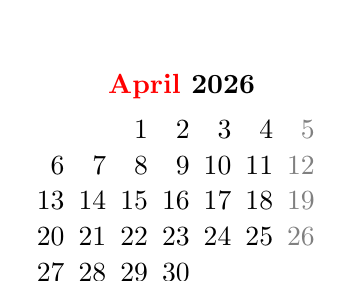
\begin{tikzpicture}[transform shape,
        every calendar/.style={
            at={(-8ex,4ex)},
            week list,
            month label above centered, 
            month text=\bfseries\textcolor{red}{\%mt} \%y0,
            if={(Sunday) [black!50]}
        }]
      \calendar [dates=\the\year-04-01 to \the\year-04-last]; 
    ];
    \end{tikzpicture}
    
        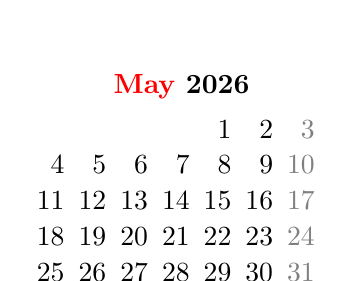
\begin{tikzpicture}[transform shape,
        every calendar/.style={
            at={(-8ex,4ex)},
            week list,
            month label above centered, 
            month text=\bfseries\textcolor{red}{\%mt} \%y0,
            if={(Sunday) [black!50]}
        }]
     \calendar [dates=\the\year-05-01 to \the\year-05-last];
       
    ];
    \end{tikzpicture}

    
    
    
    

%----------------------------------------------------------------------------------------
%	Thermo
%----------------------------------------------------------------------------------------

\section*{Thermodynamics Plan}

\begin{enumerate}
\item Claussius/Otto Cycle.
\item Phase transitions.
\item Maxwell's relations.\\
		\\
	 Less important but still important:
	\begin{itemize}
		\item Exact differentials.
		\item Third law.
		\item Porous plug problems.
	\end{itemize}
\end{enumerate}



%------------------------------------------------


%----------------------------------------------------------------------------------------
%	Thermo
%----------------------------------------------------------------------------------------

\section*{Statistical Mechanics Plan}

\begin{itemize}
\item Claussius/Otto Cycle.
\item Phase transitions.
\item Maxwell's relations.\\
		\\
	 Less important but still important:
	\begin{itemize}
		\item Exact differentials.
		\item Third law.
		\item Porous plug problems.
	\end{itemize}
\end{itemize}



%------------------------------------------------


\end{document}